\documentclass[11pt,a4paper]{article}

% --- Packages ---
\usepackage[utf8]{inputenc}
\usepackage[T1]{fontenc}
\usepackage{geometry}
\geometry{top=2.5cm, bottom=2.5cm, left=2.5cm, right=2.5cm}
\usepackage{graphicx}
\usepackage{hyperref}
\usepackage{listings}
\usepackage{xcolor}
\usepackage{booktabs}
\usepackage{float}
\usepackage{amsmath}
\usepackage{amsfonts}
\usepackage{tikz}
\usetikzlibrary{shapes.geometric, arrows.meta, positioning}

% --- Hyperref Setup ---
\hypersetup{
    colorlinks=true,
    linkcolor=blue,
    filecolor=magenta,      
    urlcolor=cyan,
    pdftitle={WhereAmI - Project Report},
    pdfpagemode=FullScreen,
}

% --- Listings Code Styling ---
\definecolor{codegray}{rgb}{0.5,0.5,0.5}
\definecolor{codepurple}{rgb}{0.58,0,0.82}
\definecolor{backcolour}{rgb}{0.95,0.95,0.92}
\definecolor{kotlinblue}{rgb}{0.12, 0.47, 0.74}
\definecolor{kotlingreen}{rgb}{0.25, 0.60, 0.30}

\lstdefinelanguage{Kotlin}{
  keywords={package, import, public, private, protected, internal, class, interface, object, fun, val, var, return, null, true, false, if, else, while, for, in, when, is, as, init, constructor, this, super, companion, data, suspend, operator},
  keywordstyle=\color{kotlinblue}\bfseries,
  ndkeywords={@Composable, @OptIn, @SuppressLint, @Test, @RunWith},
  ndkeywordstyle=\color{kotlingreen}\bfseries,
  identifierstyle=\color{black},
  sensitive=true,
  comment=[l]{//},
  morecomment=[s]{/*}{*/},
  commentstyle=\color{codegray}\itshape,
  stringstyle=\color{codepurple},
  morestring=[b]",
  morestring=[s]{"""*}{*"""}
}

\lstset{
    backgroundcolor=\color{backcolour},   
    commentstyle=\color{codegray},
    keywordstyle=\color{blue},
    numberstyle=\tiny\color{codegray},
    stringstyle=\color{codepurple},
    basicstyle=\ttfamily\footnotesize,
    breakatwhitespace=false,         
    breaklines=true,                 
    captionpos=b,                    
    keepspaces=true,                 
    numbers=left,                    
    numbersep=5pt,                  
    showspaces=false,                
    showstringspaces=false,
    showtabs=false,                  
    tabsize=2
}

\begin{document}

% ==========================================
% TITLE PAGE
% ==========================================
\begin{titlepage}
    \centering
    \vspace*{1.5cm}
    
    % Logo
    
\includegraphics[width=0.4\textwidth]{../app/src/main/res/drawable/whereami_logo.png} \\[1.5cm]
    
    {\Huge \bfseries WhereAmI}\\[0.4cm]
    {\LARGE \itshape Multiplayer geo-guessing Android application}\\[1.5cm]
    
    \textbf{\Large Course: SY43}\\[0.8cm]
    
    \vfill
    
    \textbf{Created by:}\\[0.4cm]
    Léonard GOETZ\\[0.2cm]
    Navjit KAMAL JIT\\[0.2cm]
    Pierre ZUNDEL\\[0.2cm]
    Sacha MOEBEL\\[1cm]
  
\end{titlepage}

\newpage
\tableofcontents
\newpage

% ==========================================
% SECTION 1: PROJECT SPECIFICATION
% ==========================================
\section{Project specification}

\subsection{Description of the chosen application theme}
Our mobile application \textbf{WhereAmI} is a real-time multiplayer geo-guessing game designed for friends. While popular games like \textit{GeoGuessr} use street view images from public APIs, \textbf{WhereAmI} offers a personalized experience: users challenge their friends by uploading photos they took themselves. 

In a typical gameplay scenario, a user uploads a photo from their device. The application tags the image with the user's exact geographical coordinates using the device's built-in GPS sensor. Other players in the game lobby are then tasked with finding where the photo was taken. They guess the location by placing a pin on a map. Points are computed based on the distance between the guess and the actual coordinate.

\subsection{Target users and expected use cases}
The primary target users are mobile gamers, social groups, outdoor explorers and even relatives living in different regions. Two major use cases describe the user interactions:
\begin{enumerate}
    \item \textbf{Friend group interaction:} A group of friends traveling to different locations upload photos of landmarks or hidden spots. They challenge each other to see who can guess the precise location.
    \item \textbf{Real-time lobbies :} Competitive players create group rooms and launch custom games. The application updates round statuses, images, and score sheets in real-time, allowing users to play synchronously.
\end{enumerate}

\subsection{Functional and non-functional requirements}
\subsubsection{Functional requirements}
\begin{itemize}
    \item \textbf{Authentication \& account management:} Users can sign up, log in, manage their profile details (first name, last name, username, profile picture), and reset their password using secure deep-linking (`whereami://reset-password`).
    \item \textbf{Social subsystem:} Users can search for other players, send/accept/decline friend requests and form groups.
    \item \textbf{Game creation:} Lobbies can configure games with a custom number of rounds and specific round durations (e.g., 2 hours).
    \item \textbf{Geotagged photo upload:} A player uploads a photo for a game round. The system uses the device's location sensor to capture the GPS coordinates (Latitude/Longitude) at the time of publication.
    \item \textbf{Interactive map guessing:} Opponents view the uploaded image and place a pin on an open-source interactive map (OpenStreetMap) to register their guess.
    \item \textbf{Score calculation:} Scores are automatically calculated using an exponential decay function based on the physical distance between the target and the guessed coordinates.
    \item \textbf{Real-time leaderboard:} The system tracks individual round scores and cumulative game scores, presenting them on a podium layout.
\end{itemize}

\subsubsection{Non-functional requirements}
\begin{itemize}
    \item \textbf{Real-time syncing:} Game states, picture uploads, and guess statuses must sync instantly across devices.
    \item \textbf{Security:} Database access must be restricted using Row Level Security (RLS) policies so that users can only view games and uploads belonging to their groups.
    \item \textbf{Usability:} Intuitive Compose-based layouts with clear navigation (Bottom Navigation Bar) and handling of location permissions.
\end{itemize}

\newpage

% ==========================================
% SECTION 2: CONCEPTUALIZATION OF THE APPLICATION
% ==========================================
\section{Conceptualization of the application}

\subsection{System architecture and main components}
The client application is built using Android architecture guidelines, combining \textbf{Clean Architecture} principles with the \textbf{MVVM (Model-View-ViewModel)} presentation pattern. It uses \textbf{Jetpack Compose} for UI rendering and leverages a serverless cloud infrastructure powered by \textbf{Supabase}.

\begin{figure}[H]
    \centering
    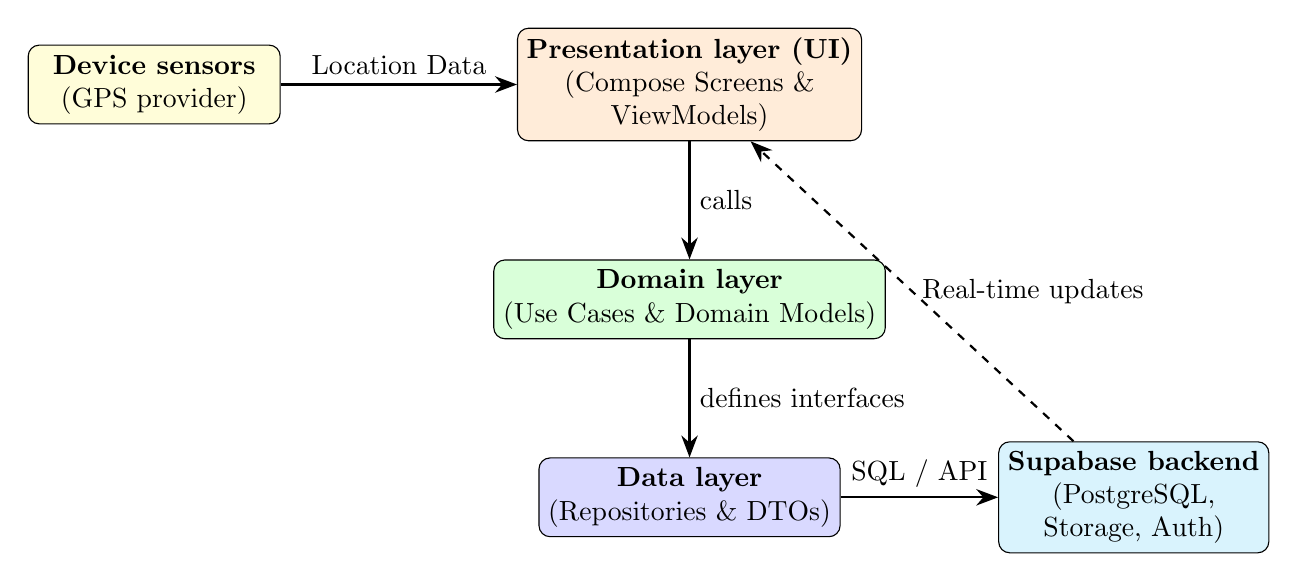
\begin{tikzpicture}[
        node distance=1.5cm,
        box/.style={draw, rectangle, rounded corners, minimum width=3.2cm, minimum height=1cm, align=center, fill=blue!10},
        arrow/.style={-{Stealth[scale=1.2]}, thick}
    ]
        % Client UI Layer
        \node (ui) [box, fill=orange!15] {\textbf{Presentation layer (UI)} \\ (Compose Screens \& \\ ViewModels)};
        
        % Domain Layer
        \node (domain) [box, below=of ui, fill=green!15] {\textbf{Domain layer} \\ (Use Cases \& Domain Models)};
        
        % Data Layer
        \node (data) [box, below=of domain, fill=blue!15] {\textbf{Data layer} \\ (Repositories \& DTOs)};
        
        % External Services
        \node (db) [box, right=2cm of data, fill=cyan!15] {\textbf{Supabase backend} \\ (PostgreSQL, \\ Storage, Auth)};
        \node (gps) [box, left=3cm of ui, fill=yellow!15] {\textbf{Device sensors} \\ (GPS provider)};
        
        % Connections
        \draw [arrow] (ui) -- (domain) node[midway, right] {calls};
        \draw [arrow] (domain) -- (data) node[midway, right] {defines interfaces};
        \draw [arrow] (data) -- (db) node[midway, above] {SQL / API};
        \draw [arrow] (gps) -- (ui) node[midway, above] {Location Data};
        \draw [arrow, dashed] (db) -- (ui) node[midway, right] {Real-time updates};
    \end{tikzpicture}
    \caption{Architecture and data flow diagram of the WhereAmI application.}
    \label{fig:architecture}
\end{figure}

The codebase is logically separated into three layers:
\begin{enumerate}
    \item \textbf{Presentation layer (UI):} Jetpack Compose functions render state-driven UI screens. The \texttt{ViewModel} classes (e.g., \texttt{RoundViewModel}) handle presentation logic, consume use cases, and expose state via Kotlin flows.
    \item \textbf{Domain layer:} Contains business logic. It defines the entities (\texttt{Game}, \texttt{User}, \texttt{Round}, \texttt{Guess}) and triggers operations via Use Cases (e.g., \texttt{SubmitGuessUseCase}). It defines repository interfaces to maintain independence from specific database technologies.
    \item \textbf{Data layer:} Implements domain repository interfaces (e.g., \texttt{SupabaseGameRepository}). It manages remote communication using Supabase clients, parsing PostgreSQL JSON payloads into Data Transfer Objects (DTOs).
\end{enumerate}

\newpage
\subsection{UML diagrams}

\subsubsection{Use case diagram}
The interaction between the client player, the GPS sensor, and the Supabase backend is illustrated below.
\begin{figure}[H]
    \centering
    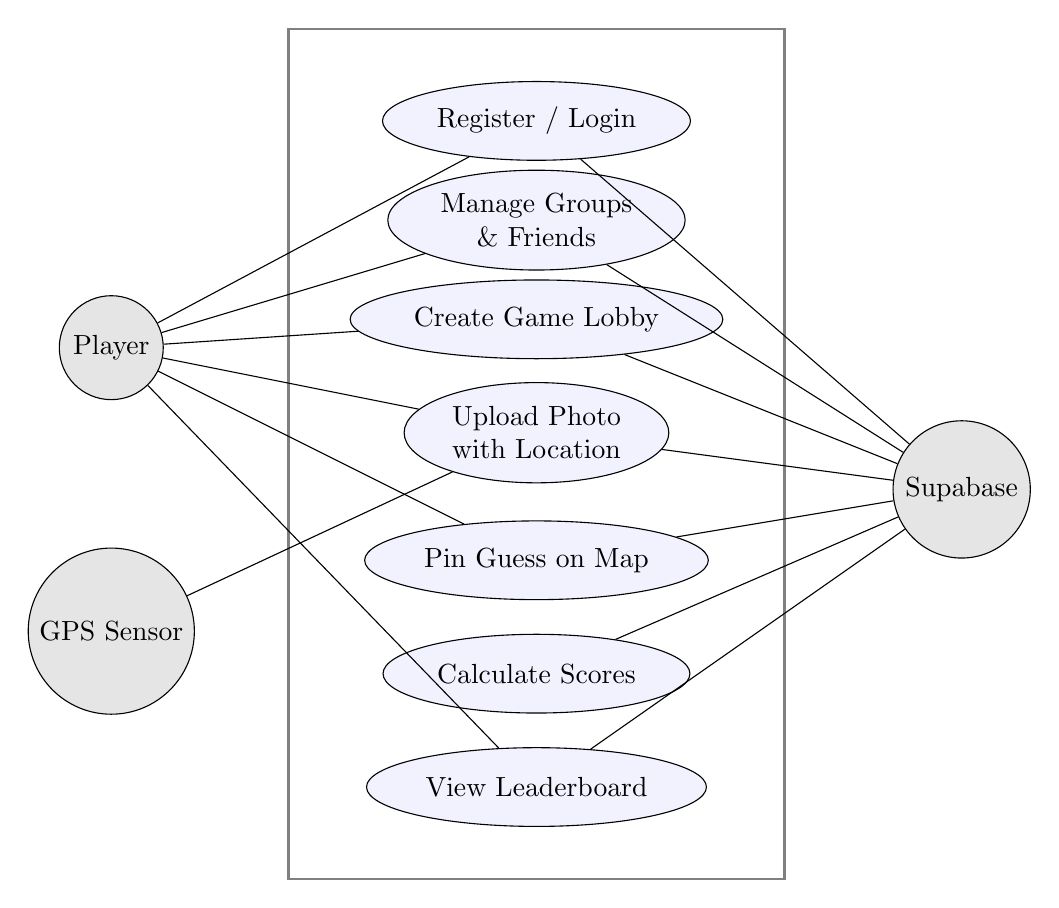
\begin{tikzpicture}[
        scale=0.9,
        actor/.style={draw, circle, minimum size=1cm, fill=gray!20},
        usecase/.style={draw, ellipse, minimum width=2.5cm, minimum height=1cm, align=center, fill=blue!5},
        arrow/.style={-}
    ]
        % Actors
        \node (player) [actor] at (-6, 0) {Player};
        \node (gps) [actor] at (-6, -4) {GPS Sensor};
        \node (backend) [actor] at (6, -2) {Supabase};

        % System Boundary
        \draw[gray, thick] (-3.5, 4.5) rectangle (3.5, -7.5);

        % Use Cases
        \node (uc1) [usecase] at (0, 3.2) {Register / Login};
        \node (uc2) [usecase] at (0, 1.8) {Manage Groups \\ \& Friends};
        \node (uc3) [usecase] at (0, 0.4) {Create Game Lobby};
        \node (uc4) [usecase] at (0, -1.2) {Upload Photo \\ with Location};
        \node (uc5) [usecase] at (0, -3.0) {Pin Guess on Map};
        \node (uc6) [usecase] at (0, -4.6) {Calculate Scores};
        \node (uc7) [usecase] at (0, -6.2) {View Leaderboard};

        % Player Connections
        \draw [arrow] (player) -- (uc1);
        \draw [arrow] (player) -- (uc2);
        \draw [arrow] (player) -- (uc3);
        \draw [arrow] (player) -- (uc4);
        \draw [arrow] (player) -- (uc5);
        \draw [arrow] (player) -- (uc7);

        % Sensor Connection
        \draw [arrow] (gps) -- (uc4);

        % Backend Connections
        \draw [arrow] (uc1) -- (backend);
        \draw [arrow] (uc2) -- (backend);
        \draw [arrow] (uc3) -- (backend);
        \draw [arrow] (uc4) -- (backend);
        \draw [arrow] (uc5) -- (backend);
        \draw [arrow] (uc6) -- (backend);
        \draw [arrow] (uc7) -- (backend);
    \end{tikzpicture}
    \caption{Use case diagram illustrating system actors and core actions.}
    \label{fig:usecase}
\end{figure}

\newpage
\subsubsection{Activity diagram}
The following diagram details the sequence of activities during a single round of the game:
\begin{figure}[H]
    \centering
    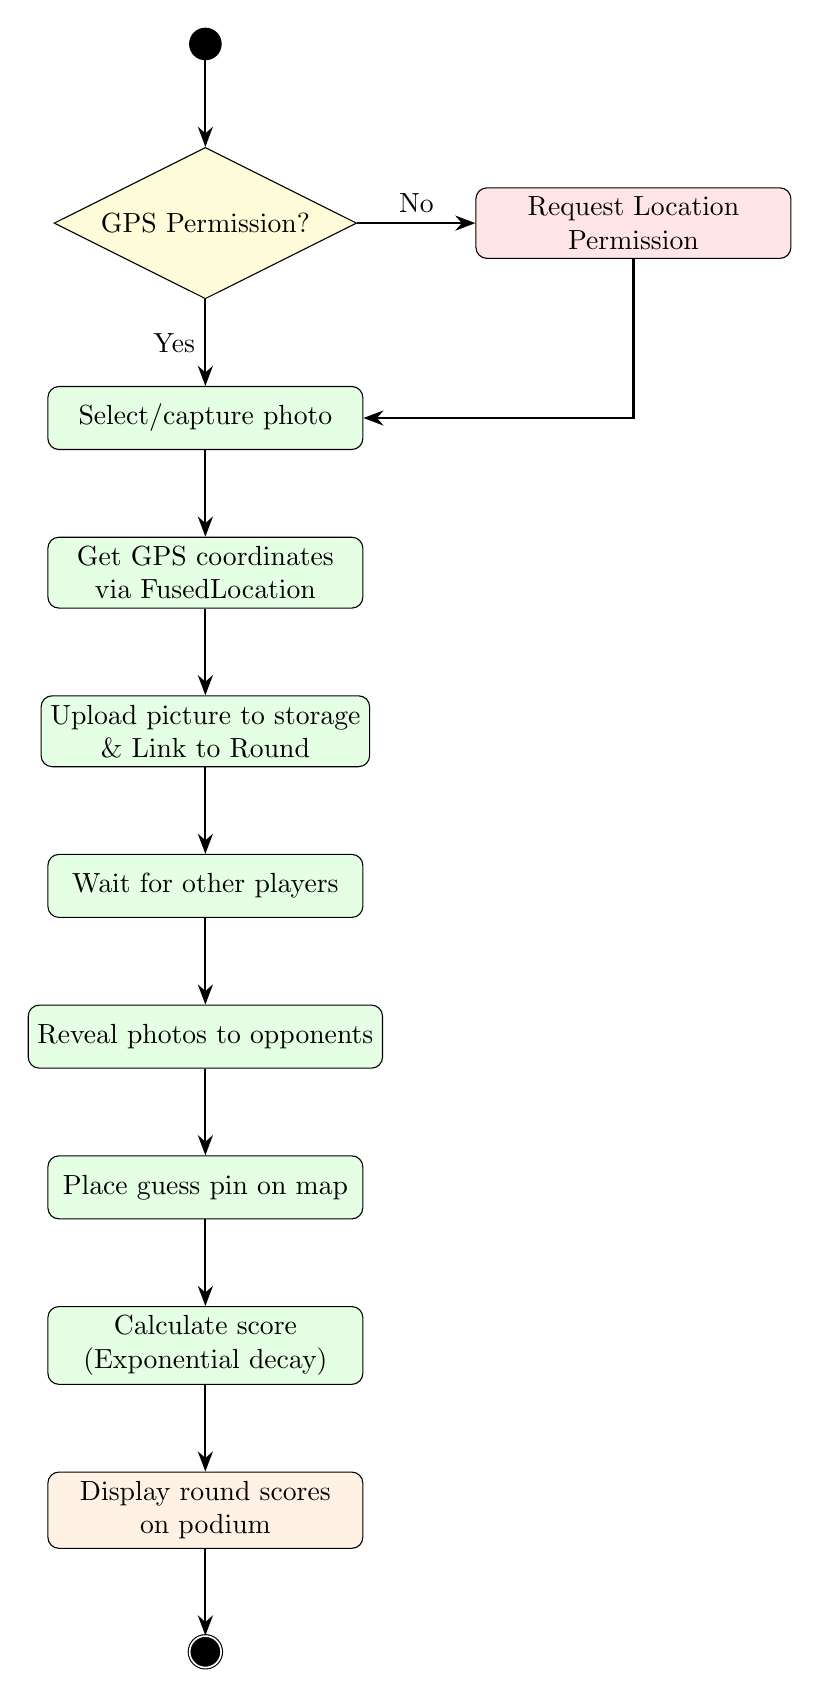
\begin{tikzpicture}[
        node distance=1.1cm,
        startstop/.style={draw, circle, fill=black, minimum size=0.4cm},
        activity/.style={draw, rectangle, rounded corners, minimum width=4cm, minimum height=0.8cm, align=center, fill=green!10},
        decision/.style={draw, diamond, aspect=2, minimum width=2.5cm, align=center, fill=yellow!15},
        arrow/.style={-{Stealth[scale=1.1]}, thick}
    ]
        \node (start) [startstop] {};
        \node (perm) [decision, below=of start] {GPS Permission?};
        \node (req_perm) [activity, right=1.5cm of perm, fill=red!10] {Request Location \\ Permission};
        \node (capture) [activity, below=of perm] {Select/capture photo};
        \node (gps_coord) [activity, below=of capture] {Get GPS coordinates \\ via FusedLocation};
        \node (upload) [activity, below=of gps_coord] {Upload picture to storage \\ \& Link to Round};
        \node (sync) [activity, below=of upload] {Wait for other players};
        
        \node (reveal) [activity, below=of sync] {Reveal photos to opponents};
        \node (guess) [activity, below=of reveal] {Place guess pin on map};
        \node (calc) [activity, below=of guess] {Calculate score \\ (Exponential decay)};
        \node (scores) [activity, below=of calc, fill=orange!10] {Display round scores \\ on podium};
        \node (stop) [startstop, below=of scores, double] {};

        \draw [arrow] (start) -- (perm);
        \draw [arrow] (perm) -- node[left] {Yes} (capture);
        \draw [arrow] (perm) -- node[above] {No} (req_perm);
        \draw [arrow] (req_perm) |- (capture);
        \draw [arrow] (capture) -- (gps_coord);
        \draw [arrow] (gps_coord) -- (upload);
        \draw [arrow] (upload) -- (sync);
        \draw [arrow] (sync) -- (reveal);
        \draw [arrow] (reveal) -- (guess);
        \draw [arrow] (guess) -- (calc);
        \draw [arrow] (calc) -- (scores);
        \draw [arrow] (scores) -- (stop);
    \end{tikzpicture}
    \caption{Activity diagram showing the lifecycle of a game round.}
    \label{fig:activity}
\end{figure}

\newpage
\subsection{Database schema}
The backend uses a relational database model implemented on PostgreSQL within Supabase. The database contains 10 tables designed to support user relationships, group structures, real-time messaging, game states, image meta-data, and score sheets.

The database layout is structured as follows:
\begin{enumerate}
    \item \textbf{users:} Stores player profile information. When a user registers in Supabase Auth, a PostgreSQL trigger automatically copies the user ID, email, and metadata into this public table.
    \item \textbf{groups \& group\_members:} Manages social groups and controls membership roles (Admin, Member).
    \item \textbf{friendships:} Holds many-to-many user associations with states like \texttt{PENDING} or \texttt{ACCEPTED}.
    \item \textbf{games:} Represents the overall match configuration, listing parameters like round counts, duration, and overall status (\texttt{CREATED}, \texttt{PLAYING}, \texttt{FINISHED}).
    \item \textbf{rounds:} Tracks individual game slices. Each round is associated with a specific duration and a set of photo uploads.
    \item \textbf{pictures:} Records picture metadata, storing the target's public image URL and the physical GPS coordinates (Latitude, Longitude) captured from the publisher's device.
    \item \textbf{guesses:} Records a player's pinned coordinate guess, including the computed physical distance in meters and the final awarded points.
    \item \textbf{game\_scores \& round\_scores:} Aggregates points to display real-time leaderboards.
\end{enumerate}

To ensure complete database integrity, structural diagrams were created during the conceptualization phase. The Conceptual Data Model (MCD) and Logical Data Model (MLD) diagrams are shown below.

\begin{figure}[H]
    \centering
    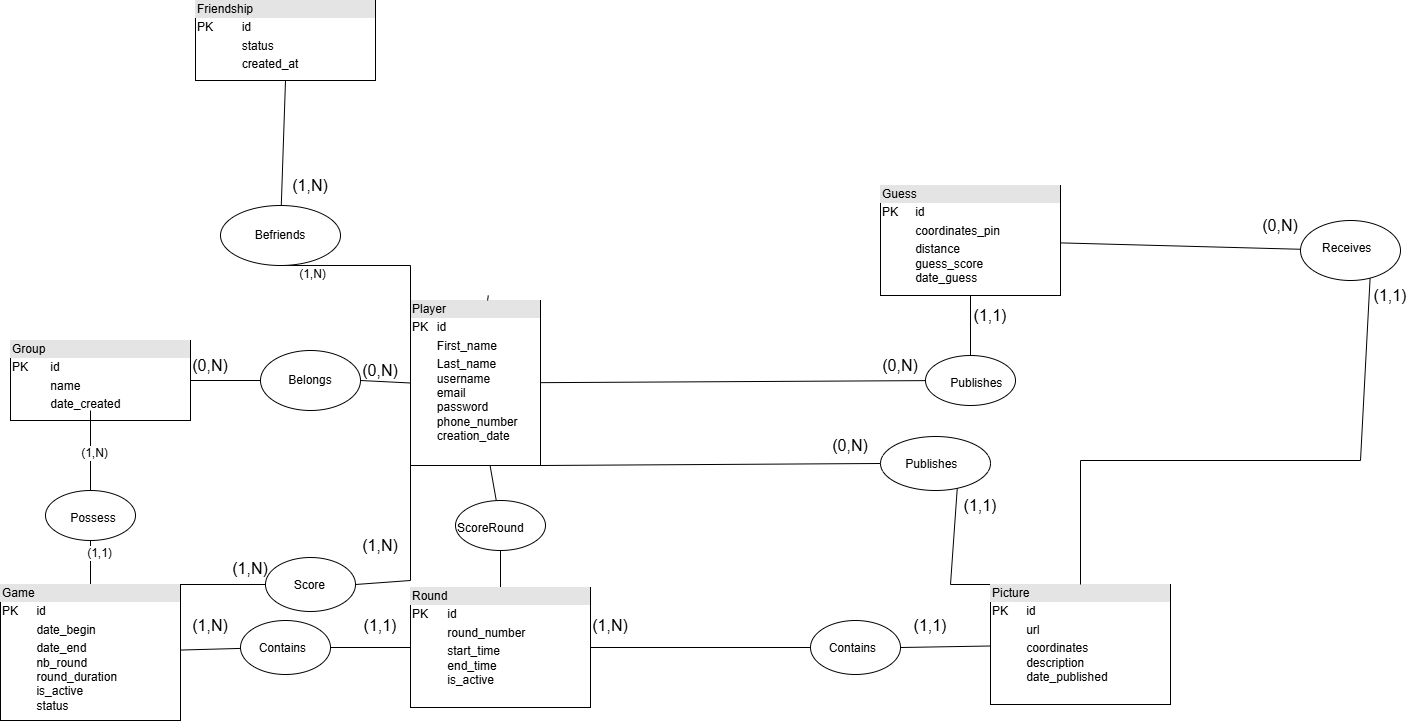
\includegraphics[width=\textwidth]{whereami-MCDFinal.drawio.png}
    \caption{Conceptual Data Model (MCD) of the WhereAmI database.}
    \label{fig:mcd}
\end{figure}

\begin{figure}[H]
    \centering
    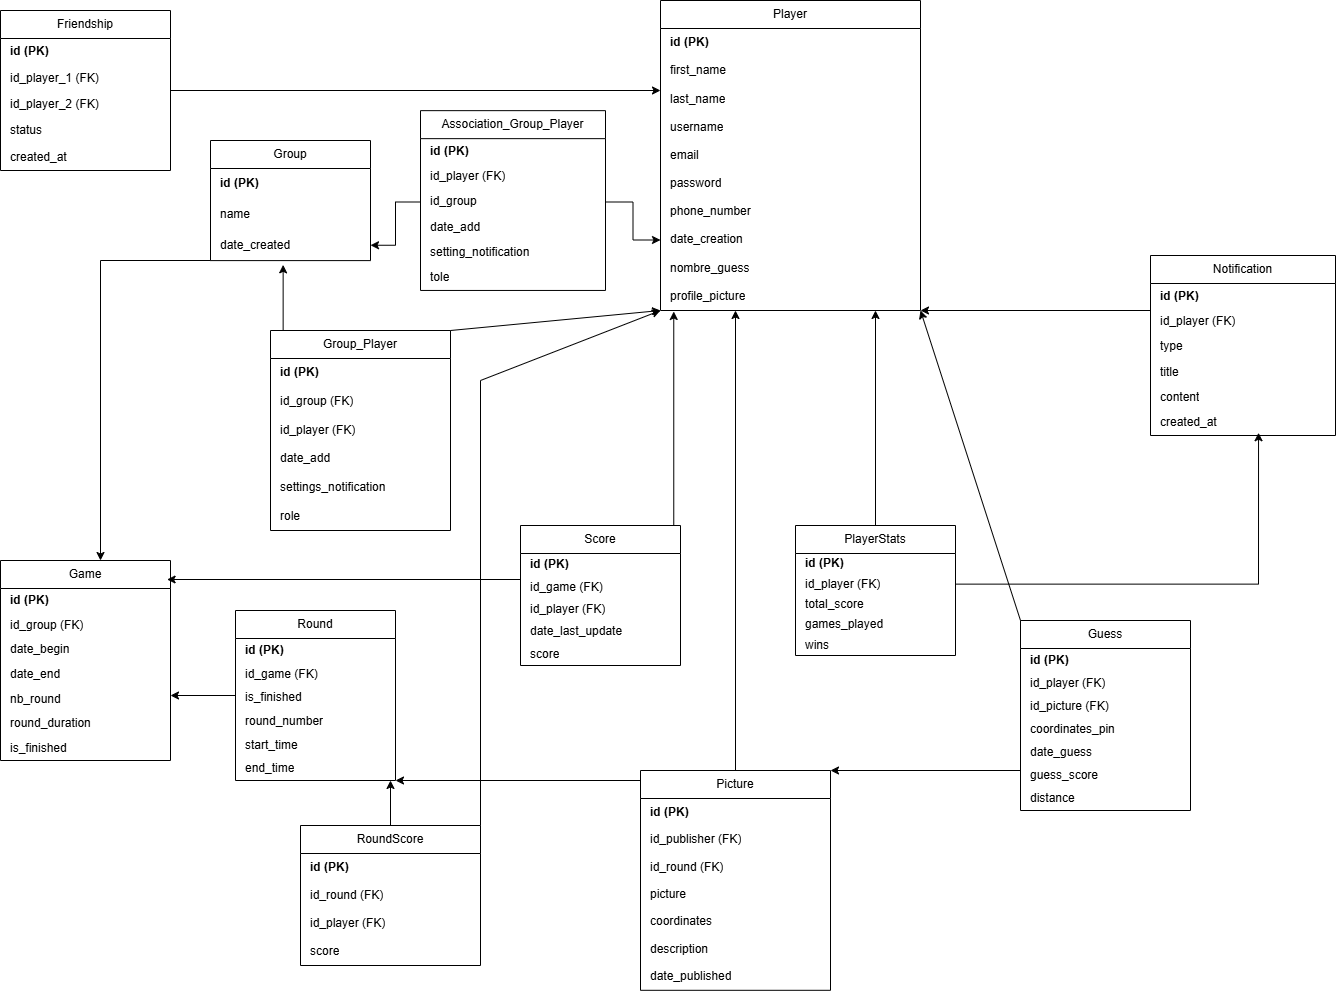
\includegraphics[width=0.95\textwidth]{mld_final.drawio.png}
    \caption{Logical Data Model (MLD) of the WhereAmI database.}
    \label{fig:mld}
\end{figure}

\newpage

% ==========================================
% SECTION 3: IMPLEMENTATION DETAILS
% ==========================================
\section{Implementation details}

\subsection{Technologies and tools used}
The implementation uses Android libraries and serverless technologies:
\begin{itemize}
    \item \textbf{Kotlin \& Jetpack Compose:} Used for core application logic and declarations of the Material Design 3 interface.
    \item \textbf{Supabase :} Provides the serverless framework, managing data storage (PostgreSQL), file storage (Supabase Storage for user pictures), and user sessions.
    \item \textbf{Ktor Client:} Used internally by Supabase for managing HTTP connections.
    \item \textbf{Google Play Services Location (21.3.0):} Integrates Android's location services to handle hardware sensors.
    \item \textbf{Osmdroid (6.1.18):} An open-source map engine used to display  maps, add markers, capture touch coordinate inputs, and display guess feedback.
    \item \textbf{Coil Compose:} An asynchronous image loading library that fetches and caches game pictures from Supabase bucket URLs.
\end{itemize}

\subsection{Key functionalities and implementation}

\subsubsection{Device location sensor integration}
The GPS sensor is accessed through the Google Play Services Location library. Before uploading a photo, the app verifies location permissions. If granted, it requests the location via \texttt{FusedLocationProviderClient}:
\begin{lstlisting}[language=Kotlin, caption={Location sensing in RoundScreen.kt}]
val fusedLocationClient = LocationServices.getFusedLocationProviderClient(context)
fusedLocationClient.getCurrentLocation(
    Priority.PRIORITY_HIGH_ACCURACY, 
    null
).addOnSuccessListener { loc: android.location.Location? ->
    if (loc != null) {
        viewModel.uploadPicture(LatLng(loc.latitude, loc.longitude), bytes)
    } else {
        viewModel.showError("Could not retrieve location. Please ensure GPS is turned on.")
    }
}
\end{lstlisting}

\newpage
\subsubsection{Dynamic scoring calculation}
The distance between the exact photo location and the player's guess is computed using the distance via \texttt{android.location.Location.distanceBetween}. The score decreases exponentially with distance:
\begin{equation}
    S = \lfloor 5000 \cdot e^{-\frac{d}{100 000}} \rfloor
\end{equation}
where $d$ is the distance in meters, and $5000$ represents the maximum possible score (perfect guess).
\begin{lstlisting}[language=Kotlin, caption={Scoring logic in SubmitGuessUseCase.kt}]
val results = FloatArray(1)
Location.distanceBetween(
    picture.location.latitude, picture.location.longitude,
    guessLatitude, guessLongitude,
    results
)
val distanceMeters = results[0].toDouble()
val score = (5000.0 * kotlin.math.exp(-distanceMeters / 100000.0)).toInt()
\end{lstlisting}

\subsubsection{Interactive map and pinning}
The Osmdroid map library is embedded in Compose using \texttt{AndroidView}. This allows users to place a pin by touching the map:
\begin{lstlisting}[language=Kotlin, caption={Map overlay interaction in RoundMapSubScreen.kt}]
val mapEventsReceiver = object : MapEventsReceiver {
    override fun singleTapConfirmedHelper(p: GeoPoint): Boolean {
        if (!uiState.isSubmittingGuess) {
            onPinLocationChanged(LatLng(p.latitude, p.longitude))
        }
        return true
    }
    override fun longPressHelper(p: GeoPoint): Boolean = false
}
val overlay = MapEventsOverlay(mapEventsReceiver)
mapView.overlays.add(overlay)
\end{lstlisting}

\subsubsection{Custom player avatars and animated podium}
To enhance personalization custom profile pictures were implemented. Avatars are uploaded as raw byte arrays and stored in a Supabase Storage bucket, with public URL links saved in the PostgreSQL \texttt{users} profiles. A reusable \texttt{UserAvatar} component displays the profile picture or dynamically generates a circular canvas featuring the player's initials on a background color derived from their username.

These avatars are integrated directly into the Osmdroid interactive maps. When a round finishes, standard map markers are replaced with circular bitmap drawables showcasing each player's avatar over their guess coordinates. Furthermore, the scoreboard leaderboard displays a 3D-style podium with gold, silver, and bronze columns. The height of these columns grows dynamically from zero to their target layout heights upon entry, powered by Jetpack Compose's \texttt{animateDpAsState} with a staggered rank-based delay:
\begin{lstlisting}[language=Kotlin, caption={Staggered podium animations in ScoresPodiumList.kt}]
val animatedHeight by animateDpAsState(
    targetValue = if (startAnimation) height.dp else 0.dp,
    animationSpec = tween(
        durationMillis = 1000,
        delayMillis = (rank - 1) * 200 // Staggered: Gold (0ms), Silver (200ms), Bronze (400ms)
    ),
    label = "podiumHeight"
)
\end{lstlisting}

\subsubsection{Security via PostgreSQL Row Level Security (RLS)}
Security policies restrict data visibility at the database level. For example, a player is only allowed to view pictures or guesses belonging to a game round they are actively participating in:
\begin{lstlisting}[language=SQL, caption={RLS policies in schema.sql}]
CREATE POLICY "Allow players to view pictures"
ON public.pictures FOR SELECT
TO authenticated
USING (
  EXISTS (
    SELECT 1 FROM public.rounds r
    JOIN public.game_scores gs ON gs.game_id = r.game_id
    WHERE r.id = round_id
    AND gs.player_id = auth.uid()
  )
);
\end{lstlisting}

\subsection{Main challenges encountered}
\begin{enumerate}
    \item \textbf{Compose and legacy view interoperability:} Osmdroid MapView was built for legacy XML layout systems. Wrapping it in an \texttt{AndroidView} and managing its lifecycle (handling recompositions and state persistence of map pins) required custom handlers.
    \item \textbf{Synchronizing game state:} As games progress, players upload images and submit guesses asynchronously. Standard database polling is inefficient and drains device batteries. The problem was solved by using Supabase Realtime Channels, which listen to table insert/update triggers and push updates to the client app.
    \item \textbf{GPS timeout \& accuracy:} Indoors or under weak network conditions, GPS sensors can return null values or take too long to obtain a lock. The app resolves this by specifying a high-accuracy priority parameter and handling null results with helpful system warnings instructing users to check their location settings.
\end{enumerate}

\newpage

% ==========================================
% SECTION 4: SCREENSHOTS AND USER INTERFACE
% ==========================================
\section{Screenshots and user interface}

\subsection{Description of the main interfaces and navigation flow}
The interfaces are structured to provide immediate feedback on game progress.
\begin{itemize}
    \item \textbf{Login / password reset screens:} Clean text input fields with real-time field validation. The reset password screen utilizes deep link listeners (`whereami://reset-password`) to automatically capture oauth recovery tokens.
    \item \textbf{Dashboard (HomeScreen):} Shows active game instances, a list of current rounds and whether the user needs to upload a picture or make guesses.
    \item \textbf{Friends and groups:} Tabbed navigation layouts showing active friends and groups. Users can invite members, create groups and games.
    \item \textbf{Round screen:} This screen manages the core gameplay loop and is split into four distinct sub-screens:
        \begin{enumerate}
            \item \textbf{Player status sub-screen:} Displays a list of player cards indicating who has uploaded a picture and who has guessed.
            \item \textbf{Picture view sub-screen:} Shows the uploaded photo that players must guess. If the user hasn't uploaded their own photo, they cannot view others.
            \item \textbf{Map view sub-screen:} Embeds the OpenStreetMap where players place their guess pin and submit it. Once a round ends, this screen displays the exact location and all player guesses.
            \item \textbf{Scores sub-screen:} Shows the final round scoreboard.
        \end{enumerate}
    \item \textbf{Podium leaderboard (ScoresPodiumList):} A custom components screen displaying the top three players on colored pillars (Gold, Silver, Bronze) and list cards for players.
\end{itemize}

\subsection{UI architecture flow}
The application navigation architecture is managed via a centralized navigation graph in \texttt{AppNavGraph.kt}. Bottom Navigation items are visible on primary screens (Home, Groups, Friends, Account) and hidden during active games to maximize map space.

\subsection{Application screenshots}
The following screenshots illustrate the main user flows and interface states of the Android application.
\newcommand{\screenshottile}[2]{%
    \begin{minipage}[t]{0.22\textwidth}
        \centering
        \includegraphics[height=0.30\textheight,keepaspectratio]{#1}\\[-0.2em]
        {\scriptsize #2}
    \end{minipage}%
}

\begin{figure}[H]
    \centering
    \screenshottile{PhotosApplication/connexionInscription.jpg}{Login / registration}
    \hfill
    \screenshottile{PhotosApplication/home.jpg}{Home}
    \hfill
    \screenshottile{PhotosApplication/groups.jpg}{Groups}
    \hfill
    \screenshottile{PhotosApplication/CreerGroupe.jpg}{Group creation}

    \vspace{0.6cm}

    \screenshottile{PhotosApplication/profileavantmaj.jpg}{Profile before update}
    \hspace{0.05\textwidth}
    \screenshottile{PhotosApplication/Profilemaj.jpg}{Profile after update}
    \hspace{0.05\textwidth}
    \screenshottile{PhotosApplication/majmotdepasse.jpg}{Password update}
    \caption{Main application screens.}
    \label{fig:application-screenshots}
\end{figure}

\newpage

% ==========================================
% SECTION 5: TESTING AND RESULTS
% ==========================================
\section{Testing and results}

\subsection{Test scenarios and validation}
Quality assurance was achieved using instrumented unit tests that validate the business layer use cases. The complete multi-user game flow was validated in \texttt{GameLogicTest.kt} using mock database repositories to isolate logic from network latency.

\begin{table}[H]
    \centering
    \small
    \caption{Core test scenarios covered in GameLogicTest.kt}
    \begin{tabular}{lll}
        \toprule
        \textbf{Test phase} & \textbf{Input / Action} & \textbf{Expected outcome} \\
        \midrule
        1. Game creation & Create game in Group with 2 rounds & Game created, Round 1 state: \texttt{CREATED} \\
        2. Media upload & Player A \& B upload photos & Upload success, locations pinned \\
        3. Guess submission & Player A guesses B's location (exact) & Score matches max: 5000 points \\
        4. Math validation & Player B guesses A's location (10km off) & Score calculated: 4539 points ($>4000$) \\
        5. Round transition & Call AdvanceRoundUseCase & Round 1 marked \texttt{FINISHED}, Round 2 created \\
        6. Leaderboard sync & Fetch game score sheets & Scores accumulated, rankings sorted \\
        \bottomrule
    \end{tabular}
    \label{tab:tests}
\end{table}

The main logic test is implemented as follows:
\begin{lstlisting}[language=Kotlin, caption={Complete game flow test (GameLogicTest.kt)}]
@Test
fun testWholeGameLogicFlow() = runBlocking {
    // 1. Create Game
    val settings = GameSettings(nbRound = 2, roundDurationMinutes = 120, dateBegin = Clock.System.now(), dateEnd = Clock.System.now())
    val createResult = createGameUseCase(groupId, settings)
    assertTrue(createResult is CreateGameResult.GameCreated)
    
    // 2. Upload pictures (Eiffel Tower and Louvre Museum coordinates)
    val locationA = LatLng(48.8584, 2.2945)
    val locationB = LatLng(48.8606, 2.3376)
    gameRepo.uploadPicture(round0.id, playerA, locationA, ByteArray(0))
    gameRepo.uploadPicture(round0.id, playerB, locationB, ByteArray(0))

    // 3. Submit guesses (A guesses B exact -> 5000 pts. B guesses A slightly off)
    val guessAResult = submitGuessUseCase(round0.id, playerA, picB, picB.location.latitude, picB.location.longitude)
    assertEquals(5000, guessAResult.getOrThrow().guessScore)

    // 4. Advance Round & Validate Scores
    val advanceResult = advanceRoundUseCase(game, round0)
    val updatedGame = advanceResult.getOrThrow()
    assertEquals(1, updatedGame.currentRoundIndex)
    assertEquals(5000, updatedGame.scoreSheets.find { it.playerId == playerA }!!.score)
}
\end{lstlisting}

\subsection{Bugs encountered and resolutions}
\begin{itemize}
    \item \textbf{Round timing accumulation:} Pre-allocated rounds in \texttt{CreateGameUseCase} accumulated leftover time if a round finished early. \\
    \textbf{Resolution:} Shifted to dynamic round creation on the fly in \texttt{AdvanceRoundUseCase.kt} so that subsequent rounds start exactly when the previous one ends, calculating duration dynamically.
    \item \textbf{Zero scores on podium:} Guess info and \texttt{PlayerBox} models lacked score fields during UI state reconstruction, resetting scores to 0 when advancing rounds. \\
    \textbf{Resolution:} Modified \texttt{AdvanceRoundUseCase.kt} to retrieve the original score-calculated guesses directly from the database using \texttt{getGuessesForRound()} before advancing.
    \item \textbf{Missing database RLS policies:} Scores did not appear on the podium because the \texttt{round\_scores} table lacked read/write policies for authenticated users. \\
    \textbf{Resolution:} Created SELECT, INSERT, and UPDATE Row-Level Security policies allowing authenticated players to manage round scores.
    \item \textbf{Timer and round transition sync:} UI timers continued running after a round was completed, and users were not transitioned to the results. \\
    \textbf{Resolution:} Monitored the round status in \texttt{RoundScreen.kt} to halt the countdown loop on \texttt{FINISHED}, auto-switched active tabs to the score view, and added a dynamic "Next Round" navigation button.
    \item \textbf{Null location exception:} FusedLocationProvider returned null under weak connectivity, causing app crashes. \\
    \textbf{Resolution:} Handled null states safely by checking GPS sensor availability first, displaying a toast message requesting user to toggle location services.
    \item \textbf{PostgreSQL schema sync issue:} Auth registrations were not linked to the public \texttt{users} profiles. \\
    \textbf{Resolution:} Created a PostgreSQL PL/pgSQL function trigger \texttt{handle\_new\_user()} that executes automatically upon inserting into the auth module.
    \item \textbf{Osmdroid gesture conflict:} Touch actions on the Compose layout conflicted with Map scroll gestures. \\
    \textbf{Resolution:} Configured the touch listener overlay in Osmdroid to consume tap gestures and update Compose states, while passing zoom events to the parent view.
\end{itemize}

\newpage

% ==========================================
% SECTION 6: CONCLUSION AND FUTURE IMPROVEMENTS
% ==========================================
\section{Potential enhancements or future developments}
While the application satisfies all project guidelines, several enhancements could expand its scope:
\begin{enumerate}
    \item \textbf{Instant messaging within lobbies and groups:} Utilizing the database's \texttt{messages} and \texttt{reactions} tables to build a persistent chat panel directly inside the game round and group lobby screens, allowing players to exchange group messages in real-time.
    \item \textbf{In-game push notifications:} Implementing background push notifications (such as notifying players when a round has been finished, when a new picture has been uploaded by a friend, or when the timer is close to expiring).
    \item \textbf{Interactive guess modification:} Allowing players to update or fine-tune their active map pins multiple times up until the round timer officially expires.
\end{enumerate}

\end{document}
